\documentclass[aspectratio=1610,14pt,t]{beamer}

% Colors
\usepackage{color}
\definecolor{mainorange}{HTML}{EC811B}
\definecolor{lightgrey}{HTML}{888888}
\definecolor{almostwhite}{HTML}{FEFEFE}

% Syntax highlighting
\usepackage{minted}
\usepackage{alltt}
\newcommand\hi[1]{{\color{mainorange} \textbf{#1}}}

% Custom unicode symbols
\usepackage{newunicodechar}
\newcommand\Warning{%
 \makebox[1.4em][c]{%
 \makebox[0pt][c]{\raisebox{.1em}{\small!}}%
 \makebox[0pt][c]{\color{red}\Large$\bigtriangleup$}}}%

\newunicodechar{⚠}{\Warning}

% Theme
\usetheme[%
  subsectionpage=progressbar,
  numbering=fraction,
  progressbar=foot,
]{metropolis}

% Customization
\usepackage{pagecolor}
\setbeamertemplate{section in toc}[sections numbered]
\setbeamerfont{title}{size=\fontsize{30}{30}}
\setbeamerfont{block title}{size=\large}
\newcommand\sep{\textcolor{lightgrey}{\rule{\linewidth}{0.05mm}}}

% Positioning
% https://tex.stackexchange.com/a/34929/13059
\def\Put(#1,#2)#3{\leavevmode\makebox(0,0){\put(#1,#2){#3}}}

% Meta
\title{Embedded Rust}
\date{2018-12-11}
\author{Raphael Nestler (@rnestler)}
\institute{Rust Zürichsee Meetup}

\begin{document}

\pgfdeclareimage[width=\paperwidth]{bg}{background-dark.pdf}
\pagecolor{almostwhite}  % Prevent speakerdeck from optimizing away the bg color
\usebackgroundtemplate{\pgfuseimage{bg}}
\maketitle

% ----------------------------------------------------------------- %

\begin{frame}[c]{println!("{:?}", Self)}
  Hi! I'm Raphael (@rnestler).

  \pause I live in Rapperswil

  \pause I work at Sensirion ({\small \url{https://sensirion.com}}).

  \pause I'm a founding member of Coredump\\hackerspace ({\small \url{https://coredump.ch}}).
\end{frame}

% ----------------------------------------------------------------- %

\begin{frame}[plain,noframenumbering]
  \frametitle{Outline}
  \setcounter{tocdepth}{1}
  \tableofcontents
\end{frame}

% ----------------------------------------------------------------- %

\pgfdeclareimage[width=\paperwidth]{bg}{background-light.pdf}
\usebackgroundtemplate{\pgfuseimage{bg}}

\section{Embedded Programming}

\begin{frame}[c]{What is an \emph{Embedded System}?}
  \begin{quote}
    A combination of computer hardware and software, and perhaps
    additional mechanical or other parts, designed to perform a dedicated
    function.
  \end{quote}
  Michael Barr. ``Embedded Systems Glossary''\footnote{\tiny\url{https://barrgroup.com/Embedded-Systems/Glossary-E\#embedded\_system}}
\end{frame}

\begin{frame}[c]{What is embedded programming?}
  \begin{itemize}
    \item Dedicated, not general purpose, µC system
    \item<1-> Baremetal
    \item<1-> Low-Level
    \item<2-> For this talk: Bare metal on Cortex-M MCUs
  \end{itemize}
\end{frame}

\begin{frame}[c]{Why do they say it's hard?}
  \begin{itemize}
    \item Harsh environment (No OS which protects you)
    \item Resource constrained (Remember dedicated?)
    \item Non-standard, Non-OSS toolchain
    \item Hard realtime requirements
    \item \ldots
  \end{itemize}
\end{frame}

\begin{frame}[c]{Why could Rust be awesome for it?}
  \begin{itemize}
    \item Zero cost abstractions!
    \item Provides safety at compiler level, not OS
    \item Expressive type system to encode constraints
  \end{itemize}
\end{frame}

\section{State of Embedded in 2018}
\begin{frame}[c]{You can use stable!}
  \begin{itemize}
    \item Previously we needed nightly for \texttt{no\_std} binaries
    \item Rust 1.6 \texttt{no\_std / libcore} gets
      introduced\footnote{\url{https://blog.rust-lang.org/2016/01/21/Rust-1.6.html}}
    \item Rust 1.27 cortex-m embedded libraries possible on stable
      \footnote{\url{https://blog.rust-lang.org/2018/10/25/Rust-1.30.0.html}}
    \item Rust 1.30 embedded binaries possible on
      stable\footnote{\url{https://blog.rust-lang.org/2018/10/25/Rust-1.30.0.html}}
    \item I recommend to use Rust 1.31 2018 edition (Released recently)
  \end{itemize}
\end{frame}

\begin{frame}[c]{You can use stable!}
%  \centering
  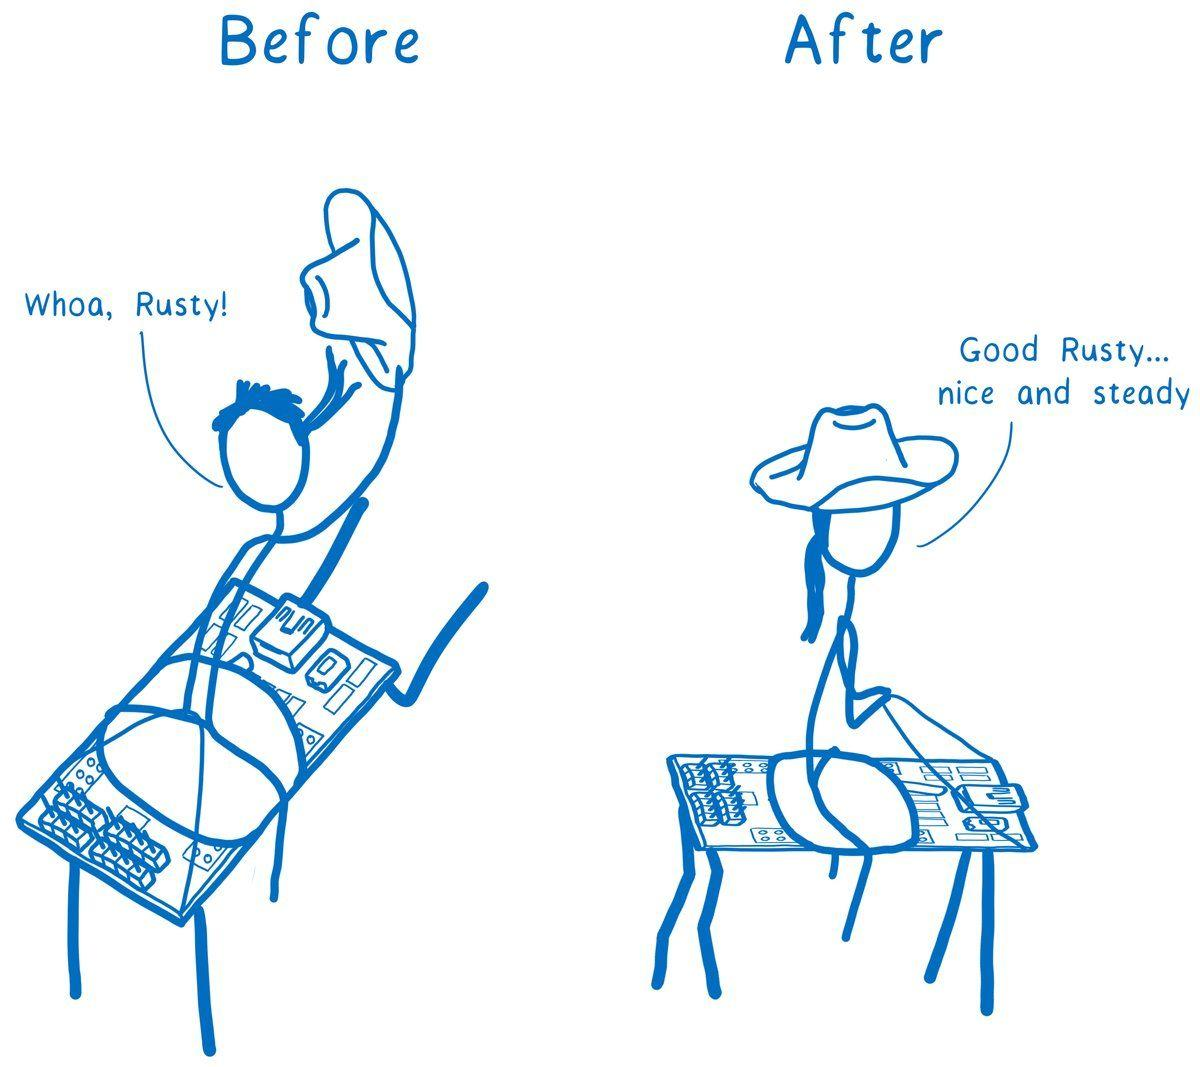
\includegraphics[width=.7\textwidth]{img/embedded-is-stable.jpg}
\end{frame}

\begin{frame}[c]{No more lib core cross compiling}
  \begin{itemize}
    \item Previously we needed to use
      xargo\footnote{\url{https://github.com/japaric/xargo}} to cross compile
      lib core
    \item Now Cortex-M targets are supported by rustup / cargo
      (thumbvxx-none-eabi)
  \end{itemize}
\end{frame}

\begin{frame}[c]{Collaborative Effort}
  \begin{itemize}
    \item Rust Embedded Working Group
    \item TODO infos
  \end{itemize}
\end{frame}

\begin{frame}[c]{More Resources}
  \begin{itemize}
    \item TODO links
  \end{itemize}
\end{frame}

\section{Getting started – STM32F3 Discovery}

\begin{frame}[c]{Prerequisites}
  \pause
  \begin{itemize}
    \item Target support by compiler
    \item Libcore compiled for the target
    \item A device crate, describes the target micro controller peripheral
    \item Runtime to setup micro controller
  \end{itemize}
\end{frame}

\begin{frame}[c]{svd2rust}
  \begin{itemize}
    \item Every Cortex-M μC vendor must provide an SVD (System View
      Descriptions) file
    \item SVD is an XML standard to describe peripheral registers
    \item svd2rust\footnote{\url{https://github.com/japaric/svd2rust}}:
      Generate Rust register maps (structs) from SVD files
    \item Done for our μC family\footnote{\url{https://github.com/japaric/stm32f30x}}
  \end{itemize}
\end{frame}

\begin{frame}[c]{Prerequisites}
  \begin{itemize}
    \item Target support by compiler (check)
    \item Libcore compiled for the target (check)
    \item A device crate, describes the target micro controller peripheral (check)
    \item Runtime to setup micro controller
  \end{itemize}
\end{frame}

\begin{frame}[c]{cortex-m, cortex-m-rt}
  \begin{itemize}
    \item The cortex-m\footnote{\url{https://github.com/rust-embedded/cortex-m}} crate gives access to common low level features of all Cortex-M devices.
    \item The cortex-m-rt\footnote{\url{https://github.com/rust-embedded/cortex-m-rt}} implements a runtime for Cortex-M μCs
  \end{itemize}
\end{frame}

\begin{frame}[c]{Prerequisites}
  \begin{itemize}
    \item Target support by compiler (check)
    \item Libcore compiled for the target (check)
    \item A device crate, describes the target micro controller peripheral (check)
    \item Runtime to setup micro controller (check)
  \end{itemize}
\end{frame}

\begin{frame}[c,fragile]{cortex-m-quickstart}
  \begin{minted}[fontsize=\footnotesize]{bash}
  $ git clone git@github.com:japaric/cortex-m-quickstart.git
  $ cd cortex-m-quickstart
  $ vim .cargo/config
  # Cortex-M4 -> thumbv7em
  # (https://en.wikipedia.org/wiki/ARM_Cortex-M)
  +[build]
  +target = "thumbv7em-none-eabihf"
  $ vim memory.x # from datasheet
  FLASH : ORIGIN = 0x00000000, LENGTH = 32K
  RAM : ORIGIN = 0x10000000, LENGTH = 6K
  \end{minted}
\end{frame}

\begin{frame}[c,fragile]{cortex-m-quickstart}
  \begin{minted}[fontsize=\footnotesize]{bash}
  # Use Beta (Or stable once 1.31 is released
  $ rustup override set beta
  $ rustc --version
  rustc 1.31.0-beta.17 (1a4f1f398 2018-11-25)
  # Install targets
  $ rustup target add thumbv7em-none-eabihf
  \end{minted}
\end{frame}

\begin{frame}[c,fragile]{Hello World using semi hosting\footnote{\url{http://blog.japaric.io/quickstart}}}
  \begin{minted}[fontsize=\footnotesize]{bash}
  $ cargo install cargo-generate
  $ cargo build --release --example hello
  # jlink.cfg
    interface jlink
    transport select swd
  # lpc11xx.cfg
  # NXP LPC11xx Cortex-M0 with at least 1kB SRAM
  set CHIPNAME lpc11xx
  set CHIPSERIES lpc1100
  if { ![info exists WORKAREASIZE] } {
    set WORKAREASIZE 0x400
  }
  source [find target/lpc1xxx.cfg]
  adapter_khz 4000
  \end{minted}
\end{frame}

\begin{frame}[c,fragile]{Hello World using semi hosting}
  \begin{minted}[fontsize=\footnotesize,breaklines]{bash}
  $ openocd -f jlink.cfg -f lpc11xx.cfg -c 'init; reset; halt'
  # separate shell
  $ arm-none-eabi-gdb target/thumbv6m-none-eabi/release/examples/hello
  (gdb) c
  # You should see "Hello, World" in the openocd console
  \end{minted}
\end{frame}

\begin{frame}[c,fragile]{Hello World explained}
  \begin{minted}[fontsize=\small]{rust}
...
use cortex_m_semihosting::hio;
...
fn main() {
    let mut stdout = hio::hstdout().unwrap();
    writeln!(stdout, "Hello, world!").unwrap();
}
  \end{minted}
\pause Semi hosting: Kind of ``system calls'' for the debugger
  \begin{itemize}
    \item Break point
    \item Content in register defines which function
    \item Debugger reads memory
  \end{itemize}
\end{frame}

\begin{frame}[c]{Demo time! --- Hello World}
\end{frame}


\section{Other Notable Projects}

\begin{frame}[c]{\url{https://www.tockos.org/}}
  \centering
  
\includegraphics[width=.8\textwidth]{img/tock.png}

  \begin{quote}
    An embedded operating system designed for running multiple concurrent,
    mutually distrustful applications on low-memory and low-power
    microcontrollers.
  \end{quote}
\end{frame}

\begin{frame}[c]{tockos}
  \begin{itemize}
    \item Uses ``capsules'' for kernel component isolation
    \item Memory Protection Units (MPU) based isolation for processes
  \end{itemize}
\end{frame}


\section{Future}

\begin{frame}[c]{More targets}
  \begin{itemize}
    \item Currently only Cortex-M are well supported
    \item Cortex-R
    \item MSP430
    \item RISCV
    \item<2-> AVR? There exits an LLVM and Rust compiler fork for it.
    \item<2-> ESP32? Currently people experiment compiling Rust to C and then
      to the ESP\ldots
  \end{itemize}
\end{frame}

\begin{frame}[c]{Ecosystem stabilization}
  \begin{itemize}
    \item Currently still a lot of moving pieces (svd2rust, cortex-m crates,
      device crates, ...)
    \item Slowing down since the Rust 2018 edition is released
  \end{itemize}
\end{frame}

\begin{frame}[c]{2019 Wishlist}
  \begin{itemize}
    \item The Rust Embedded Working Group needs our input
    \item \url{https://github.com/rust-embedded/wg/issues/256}
  \end{itemize}
\end{frame}

% ----------------------------------------------------------------- %

{
\setbeamertemplate{footline}{}
\pgfdeclareimage[width=\paperwidth]{bg}{background-inverted.pdf}
\usebackgroundtemplate{\pgfuseimage{bg}}
\begin{frame}[standout]
  \begin{centering}
    {\Huge Thank you!}\\
    {\normalsize \url{https://coredump.ch}}\\
  \end{centering}
  {\small Slides: \url{https://github.com/rust-zurichsee/meetups/}}\\
  \vspace{3cm}
\end{frame}
}
\end{document}
